\documentclass[11pt]{article}

\usepackage{listings}
\usepackage{xcolor}
\usepackage{graphicx}
\usepackage[top=2cm,bottom=2cm,left=3cm, right=3cm]{geometry}
\usepackage{float}

\lstset{
basicstyle=\scriptsize\tt,
  backgroundcolor=\color{gray!10},
  commentstyle=\color{green!60!black},
  keywordstyle=\color{blue},
  stringstyle=\color{orange},
  numbers=left,
  numbersep=5pt,
  numberstyle=\tiny\color{gray},
}



\title{Report on Partitioning Clustering and  Energy Forecasting}
\newcommand{\name}{Hasanur Rahman Mohammad}
\newcommand{\studentID}{w1780941}
\newcommand{\moduleCode}{5DATA002W}
\newcommand{\tutor}{Mahmoud Aldraimli}
\newcommand{\seminarGroup}{5CS01}
\setlength{\parindent}{0pt}

\begin{document}
\begin{titlepage}

    \center
    {\LARGE\bfseries Report on Partitioning Clustering and Energy Forecasting}
    \\ [2cm]
    \begin{flushleft}
        \textbf{Name: }\name \\
        \textbf{Student ID: }\studentID \\[0.5cm]
        \textbf{Module Code: }\moduleCode \\
        \textbf{Tutor: }\tutor \\
        \textbf{Seminar Group: }\seminarGroup\\
    \end{flushleft}

\end{titlepage}

\tableofcontents
\newpage

\section{Partitioning Clustering}
\subsection{Pre-Processing the data}
For this task we were given a vehicle.xmls file containing \textbf{846} samples, with \textbf{19} different attributes
including the \textbf{'Class'}. However, as the goal is to perform k-means clustering on the data, an unsupervised learning algorithm,
it is required to remove the \textbf{'Class'} column as the model will classify the data on its own. I also removed the 'Sample' column as it will
affect the next pre-processing tasks, scaling and outlier removal.\\

When it comes to the order, I chose to remove the outliers first as they seemed to negatively affect the clustering results if I scaled the data before removing them.
To find the outliers I found the \textbf{z-score} for each of the samples and then removed any samples with a \textbf{z-score} than \textbf{3} and less than \textbf{-3}.

\subsection{Finding the best k using: Nblust, Elbow method, Gap statistics and sillhoutte methods}

\subsubsection{Nblust}
As shown below, Nbclust says the best number of clusters is 3. Considering the original number of classes is 4 I believe that this is a good result.
\begin{lstlisting}
* Among all indices:                                                
* 6 proposed 2 as the best number of clusters 
* 12 proposed 3 as the best number of clusters 
* 1 proposed 6 as the best number of clusters 
* 1 proposed 8 as the best number of clusters 
* 1 proposed 11 as the best number of clusters 
* 1 proposed 12 as the best number of clusters 
* 2 proposed 15 as the best number of clusters 

                   ***** Conclusion *****                            
 
* According to the majority rule, the best number of clusters is  3 
\end{lstlisting}

\subsubsection{Elbow Method}
\begin{figure}[H]
  \centering
  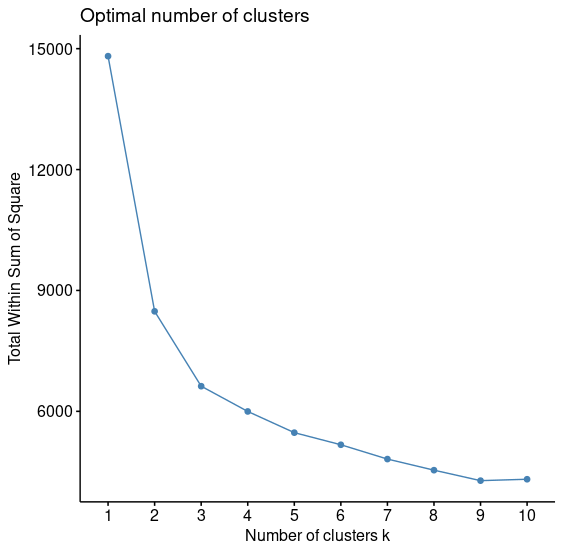
\includegraphics[width=0.45\textwidth]{~/Documents/rcw/images/Rplot.png}
  \caption{Elbow method plot}
\end{figure}

The Elbow method uses the \textbf{WCSS(within-cluster sums of squares)} which measueres how close data points are in respect of their cluster centers.
Based on the plot above, the reccomended number of clusters is \textbf{3} as that is where the results begin to flatten out slowly
indicating that increasing the clusters anymore will not result in any increase in performance.

\subsubsection{Gap Statistics}
\begin{figure}[H]
  \centering
  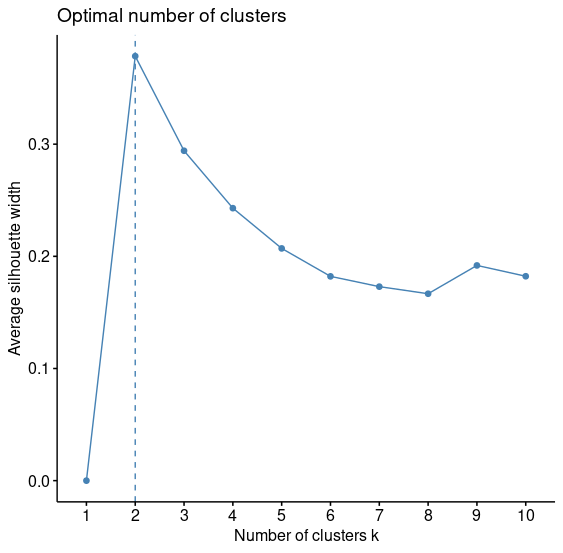
\includegraphics[width=0.5\textwidth]{~/Documents/rcw/images/Rplot01.png}
  \caption{Gap statistics plot}
\end{figure}

The Gap statistics also uses the \textbf{WCSS} to calculate the best number of clusters to use.  
However, the reccomended number of clusters in this case is \textbf{2}, knowing that the orignal data set has \textbf{4} possible classes,
we can conclude that this result is worse than what we got with the elbow method which was \textbf{3}.

\subsubsection{Sillhoutte  Method}
\begin{figure}[H]
  \centering
  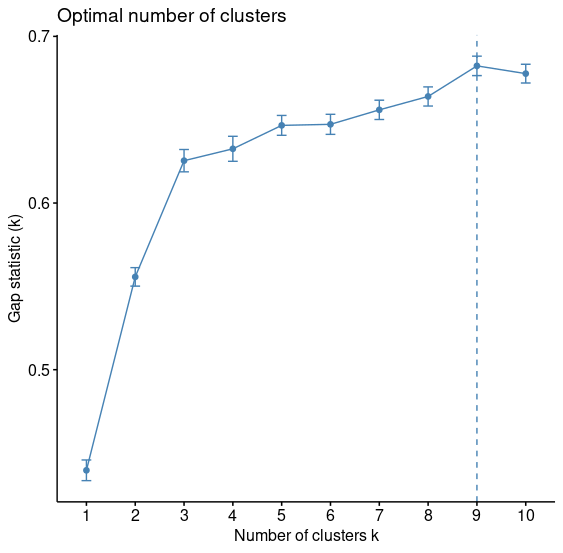
\includegraphics[width=0.5\textwidth]{~/Documents/rcw/images/Rplot02.png}
  \caption{Sillhoutte method plot}
\end{figure}

The sillhoutte plot shows how similar a data point is to its own cluster using the \textbf{sillhuotte score}, this is a value 
that ranges from -1 and 1, with values closer to -1 meaning the data point should be in another cluster and the closer the value is to 1 meaning the current cluster is a good fit for the data point
This is where things get interesting, based on the plot above \textbf{9} is the reccomended number of clusters. This is significantly higher
than any of the other results from the other evaluation methods,
I made to sure to run the model several times checking if there were errors with the code, but it gave \textbf{9} as the ouput everytime. This is by far the worst result as the orignal data set has \textbf{4} classes

However as shown later in the report, after running the evaluation tools for the data that had \textbf{PCA} done on it. The results for the sillhoutte plot were 
a lot more controlled and matched the other evaluation methods as well. This led me to believe that having a data set that is too multi-demensional led to an extreme result for the sillhoutte plot.

\newpage
\subsection{K-means Clustering investigation}
\subsubsection{Discussing the K-means outputs}
Using the results from the evaluation methods, I decided to go for \textbf{k=3}, as both \textbf{Nbclust} and the \textbf{Elbow Method} \
gave a result of the best \textbf{k} being \textbf{3}.
Below you can see the plot made from the clustering, without looking at the output data you can see a clear distinction between the clusters where there is 
no overlapping

\begin{figure}[H]
  \centering
  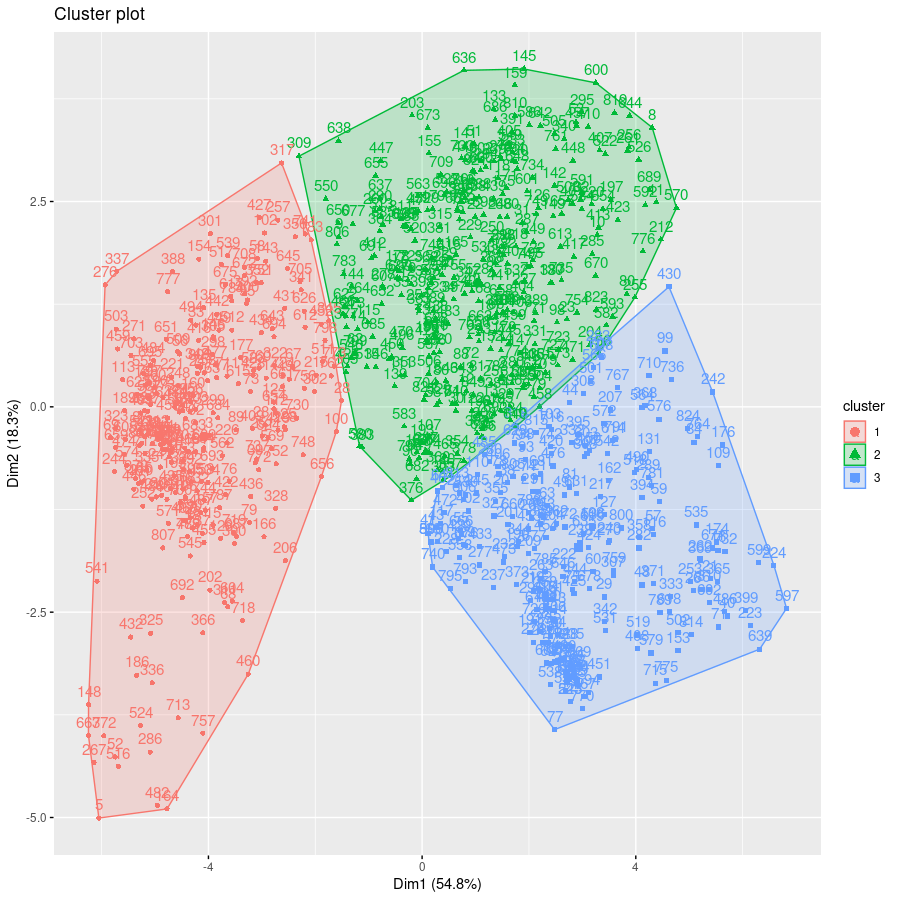
\includegraphics[width=0.8\textwidth]{~/Documents/rcw/images/Rplot05.png}
  \caption{Clustering plot}
\end{figure}

Below are the kmeans output for the clustering attempt with \textbf{k=3}. You can see that the sizes of each cluster is evenly distributed
which implies that the clustering did not favour or ingnore any specific cluster. 
The \textbf{BSS(between sums of squares)} in this clustering is \textbf{8189.91} while the \textbf{WSS(within cluster sums of squares)} is \textbf{6624.09}. 
The ratio of the \textbf{BSS} and the \textbf{TSS(total sums of squares)} is \textbf{55.3\%}, this number shows how well the clusters are seperated from each other where a higher value 
means that clusters are well seperated and a lower value means the clusters are not well defined.

To further investigate whether it was possible to get a lower \textbf{WSS} and a higher \textbf{BSS}, I run the clustering with \textbf{k=2} which was the second most reccomended value of \textbf{k} by the automated tools,
I concluded that \textbf{k=3} was indeed the best number of clusters as the \textbf{BSS} was higher while the the \textbf{WSS} was lower in the clustering attempt with \textbf{k=2}.
\\
\\
\lstinputlisting{tools.txt}

\newpage
\subsubsection{Sillhoutte Plot}

The sillhouette plot shows how well the clustering is taking place and it will calucalte the average distance between the clusters.
In practice the plot displays how close each point in one cluster is to poins in the neighbouring clusters.
The \textbf{average width score} indicates how well the samples are well clustered, it ranges from \textbf{1} to \textbf{-1} where a score close to \textbf{1} means the samples are well matched to their own cluster while 
a score closer to \textbf{-1} means the samples are poorly matched to their own clusters, and a score clsoe to \textbf{0} means the samples are more ambiguously placed and could be in another cluster.

\begin{figure}[H]
  \centering
  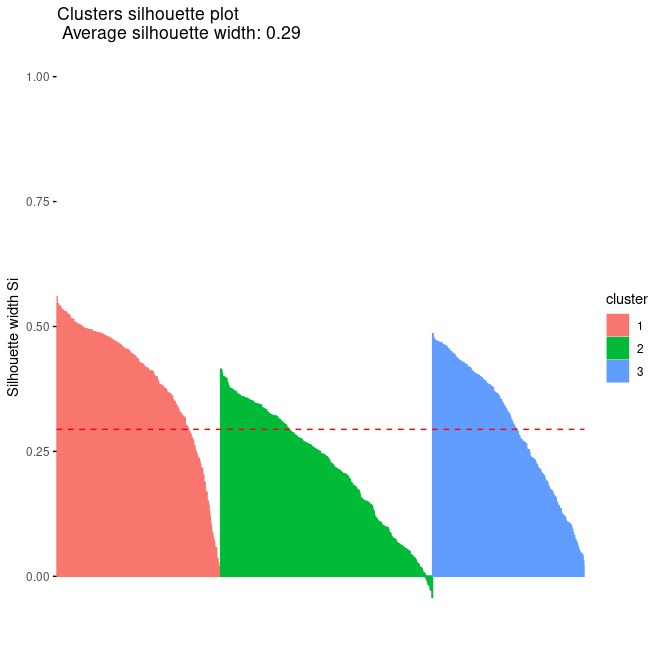
\includegraphics[width=0.5\textwidth]{~/Documents/rcw/images/Rplot06.png}
  \caption{Sillhoutte plot}
\end{figure}

From the plot above you can see that the \textbf{average width score} is \textbf{0.29}, being a positive value we can say that the clusters are moderately accurate, but as the maxmimum score is \textbf{1} there can still be some improvements in the clustering
to achieve a better \textbf{average width score}

\subsection{K-means Clustering with PCA}
\subsubsection{Creating the new dataset with PCA}
Below I have khown the \textbf{eigenvalues}, the \textbf{eigenvectors}, and the \textbf{cumulative score} per principle component. 
To make the new transformed dataset we want to use the PCs with at least a \textbf{cumulative score} of \textbf{\textgreater 92\%}
I decided to use the first \textbf{6 PCs} as they gave a total score of \textbf{0.94}
\begin{lstlisting}
> eigenvalues
 [1] 9.8655415144 3.3026315672 1.2050866140 1.1255984677 0.8773731809 0.6636174794
 [7] 0.3374343341 0.2274918343 0.1176165632 0.0871789864 0.0607683889 0.0450646831
[13] 0.0292070985 0.0213994038 0.0150961795 0.0123913361 0.0061400710 0.0003622977

> eigenvectors
                     PC1         PC2         PC3          PC4         PC5          PC6
Comp         -0.27099550  0.08819711 -0.03979285 -0.142474274 -0.15979926  0.219704493
Circ         -0.28538005 -0.14799378 -0.19761320  0.023348077  0.12602923 -0.019390179
D.Circ       -0.30078375  0.04064437  0.07450874 -0.104513476  0.07338676  0.000941066
Rad.Ra       -0.27595481  0.19284625  0.04085638  0.244080006 -0.12620414 -0.153234232
Pr.Axis.Ra   -0.10790106  0.24598582 -0.10092681  0.611908838 -0.05646656 -0.599471567
Max.L.Ra     -0.18693783  0.06836380 -0.10600156 -0.255241647  0.70801896 -0.255529947
Scat.Ra      -0.30925633 -0.07715243  0.10748098  0.001027495 -0.09117998  0.078463678
Elong         0.30718493  0.01853683 -0.09109269 -0.071391309  0.08547550 -0.061072204
Pr.Axis.Rect -0.30618660 -0.09004872  0.10605368 -0.025003047 -0.08566679  0.087748728
Max.L.Rect   -0.27419519 -0.13582051 -0.20286313 -0.052151262  0.25259264 -0.012583332
Sc.Var.Maxis -0.30244511 -0.07264590  0.13477043  0.057153180 -0.15616630  0.103440122
Sc.Var.maxis -0.30676191 -0.08004640  0.10787776  0.004398469 -0.12508727  0.106371087
Ra.Gyr       -0.25860012 -0.21823056 -0.21386460  0.068595328  0.01184258 -0.063754044
Skew.Maxis    0.06158617 -0.50300209  0.06768991  0.125377302 -0.13879190 -0.159605991
Skew.maxis   -0.03877299  0.02950349 -0.55339412 -0.517610761 -0.48274633 -0.382718195
Kurt.maxis   -0.05921378  0.09616696  0.68221125 -0.400234808 -0.09248124 -0.471711647
Kurt.Maxis   -0.04751059  0.50763917 -0.07208105  0.027069843 -0.17449701  0.240919678
Holl.Ra      -0.09728514  0.50329529 -0.03870066 -0.089901222  0.12059247  0.082978199
                     PC7          PC8          PC9        PC10        PC11
Comp          0.25075003 -0.762917498  0.336727260 -0.17080380  0.06059915
Circ         -0.38184560 -0.084996844  0.048161956  0.14521912 -0.06103582
D.Circ        0.10924250  0.307560350  0.369297550  0.09330027  0.74865950
Rad.Ra        0.13812347  0.062362314  0.159039213 -0.02487175 -0.17932432
Pr.Axis.Ra    0.06368508 -0.146618654  0.033075197  0.08677308  0.04900671
Max.L.Ra      0.40902849 -0.032642651 -0.227739119 -0.25103768 -0.10840290
Scat.Ra       0.09891112  0.092046874 -0.128654451  0.10439303 -0.14948976
Elong        -0.10476915 -0.225039791  0.263923313  0.02991565 -0.09895280
Pr.Axis.Rect  0.09681861  0.043426157 -0.071150433  0.18287483 -0.26837448
Max.L.Rect   -0.36733465 -0.241378159 -0.121107876  0.50017751  0.09455120
Sc.Var.Maxis  0.11234218  0.149165987 -0.129154922 -0.16972307  0.03485767
Sc.Var.maxis  0.08604684  0.045421860 -0.102778876  0.11442449 -0.24325771
Ra.Gyr       -0.45586499  0.112011651  0.148879282 -0.69204782 -0.05867687
Skew.Maxis    0.11079493 -0.298664862 -0.505836049 -0.11269997  0.40780344
Skew.maxis    0.12381756  0.128361642 -0.070226350  0.07170181 -0.02036668
Kurt.maxis   -0.31638913 -0.134628700  0.005249849 -0.04532918 -0.03440818
Kurt.Maxis   -0.18582252 -0.098767436 -0.460060564 -0.18269431  0.16137526
Holl.Ra      -0.18385202 -0.002257517 -0.204524578  0.01863833  0.12215130
                     PC12        PC13         PC14         PC15         PC16
Comp          0.016236215 -0.15538799 -0.084941797 -0.009893937  0.014731452
Circ         -0.108002512 -0.02379761  0.200359434 -0.411699600  0.633197650
D.Circ        0.027236923  0.23107314 -0.032038645 -0.128176485 -0.032941366
Rad.Ra       -0.148278795  0.02028449  0.782962301 -0.002680653 -0.262185162
Pr.Axis.Ra    0.061511729  0.03176897 -0.360686574  0.022171363  0.091207086
Max.L.Ra     -0.103284857  0.09369549 -0.004005999 -0.047699349  0.023924621
Scat.Ra       0.114239242 -0.02130040 -0.070286104 -0.106776285  0.005784063
Elong         0.155162263  0.75286275  0.157069120  0.228858568  0.132825704
Pr.Axis.Rect  0.272369519  0.30540490 -0.201563990 -0.167283715 -0.290260077
Max.L.Rect   -0.201414962 -0.03380300 -0.013996509  0.370105120 -0.376075706
Sc.Var.Maxis -0.228758252  0.06412845 -0.026516516  0.694529334  0.411479615
Sc.Var.maxis  0.177853616  0.28399252 -0.085543400 -0.046373620  0.145074045
Ra.Gyr        0.153739469  0.03885792 -0.107040664  0.039303314 -0.249704673
Skew.Maxis    0.220683275  0.09807688  0.277643886 -0.073168084 -0.021263745
Skew.maxis    0.001322677 -0.01515260  0.002919287  0.032651291  0.017641831
Kurt.maxis   -0.087563183 -0.01891627 -0.022107399 -0.022609384  0.002337621
Kurt.Maxis   -0.385070902  0.34206081 -0.073483280 -0.224113793 -0.089715206
Holl.Ra       0.697685477 -0.19114605  0.188619261  0.198088827  0.123427696
                      PC17          PC18
Comp          0.0022871138 -0.0001888306
Circ          0.1935606420  0.0189798203
D.Circ       -0.0338082604 -0.0095717960
Rad.Ra        0.0060687302 -0.0275176970
Pr.Axis.Ra   -0.0091405437  0.0177603416
Max.L.Ra     -0.0048404910 -0.0083581152
Scat.Ra      -0.3857289906  0.7909901632
Elong        -0.0570308312  0.2237899607
Pr.Axis.Rect  0.6548967453 -0.0151607986
Max.L.Rect   -0.1025905067 -0.0266527364
Sc.Var.Maxis  0.2336432149  0.0416825198
Sc.Var.maxis -0.5542304543 -0.5644496563
Ra.Gyr       -0.0737884732  0.0031786081
Skew.Maxis    0.0234042984 -0.0068080750
Skew.maxis    0.0046042860 -0.0030669415
Kurt.maxis   -0.0007617607 -0.0075237217
Kurt.Maxis   -0.0118304320  0.0341259519
Holl.Ra       0.0432842111 -0.0094922864


> summary(pca_data)
Importance of components:
                          PC1    PC2     PC3     PC4     PC5     PC6     PC7     PC8
Standard deviation     3.1409 1.8173 1.09776 1.06094 0.93668 0.81463 0.58089 0.47696
Proportion of Variance 0.5481 0.1835 0.06695 0.06253 0.04874 0.03687 0.01875 0.01264
Cumulative Proportion  0.5481 0.7316 0.79851 0.86105 0.90979 0.94666 0.96540 0.97804
                           PC9    PC10    PC11   PC12    PC13    PC14    PC15    PC16
Standard deviation     0.34295 0.29526 0.24651 0.2123 0.17090 0.14629 0.12287 0.11132
Proportion of Variance 0.00653 0.00484 0.00338 0.0025 0.00162 0.00119 0.00084 0.00069
Cumulative Proportion  0.98458 0.98942 0.99280 0.9953 0.99692 0.99811 0.99895 0.99964
                          PC17    PC18
Standard deviation     0.07836 0.01903
Proportion of Variance 0.00034 0.00002
Cumulative Proportion  0.99998 1.00000
\end{lstlisting}
\\
\subsection{Finding the best k for PCA dataset using: Nblust, Elbow method, Gap statistics and sillhoutte methods}

\subsubsection{Nblust}
The results for \textbf{Nbclust} while using the newly made dataset using \textbf{PCA} were not different from the orignal k-means clustering attempt using the orignal dataset. 
Nbclust still says the best number of clusters is \textbf{3}.
\begin{lstlisting}
* Among all indices:                                                
* 7 proposed 2 as the best number of clusters 
* 10 proposed 3 as the best number of clusters 
* 1 proposed 4 as the best number of clusters 
* 2 proposed 6 as the best number of clusters 
* 2 proposed 9 as the best number of clusters 
* 2 proposed 15 as the best number of clusters 

                   ***** Conclusion *****                            
 
* According to the majority rule, the best number of clusters is  3 
\end{lstlisting}

\subsubsection{Elbow Method}
\begin{figure}[H]
  \centering
  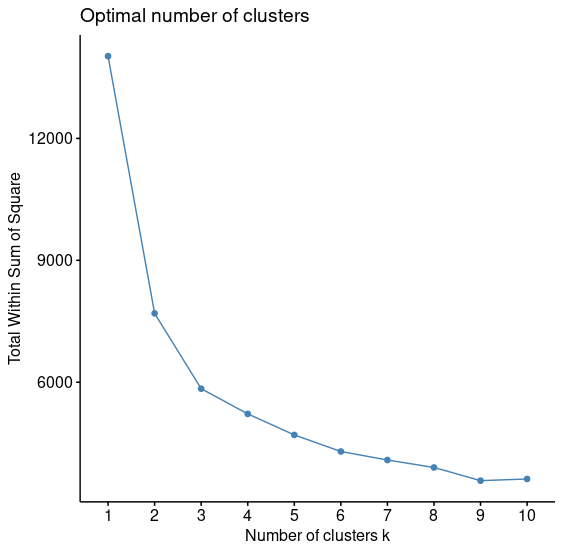
\includegraphics[width=0.5\textwidth]{~/Documents/rcw/images/Rplot07.png}
  \caption{Elbow method plot}
\end{figure}

The \textbf{elbow method} is not showing new reults and also says the reccomended number of clusters is still \textbf{3}.
\subsubsection{Gap Statistics}
\begin{figure}[H]
  \centering
  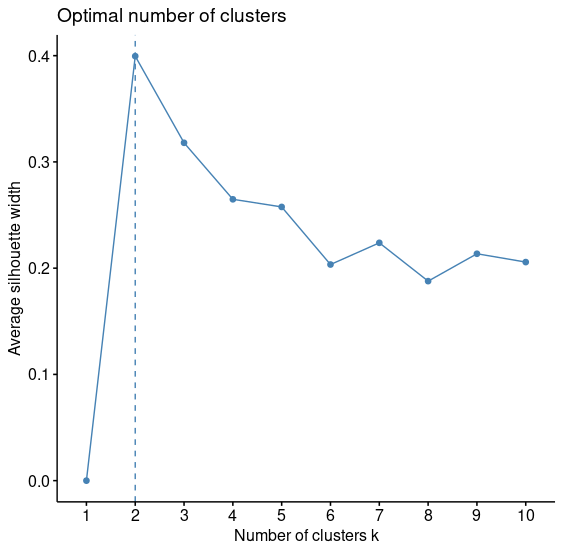
\includegraphics[width=0.5\textwidth]{~/Documents/rcw/images/Rplot08.png}
  \caption{Gap statistics plot}
\end{figure}

The \textbf{gap statistics} also still says the reccomended number of clusters is still \textbf{2}.

\subsubsection{Sillhoutte  Method}
\begin{figure}[H]
  \centering
  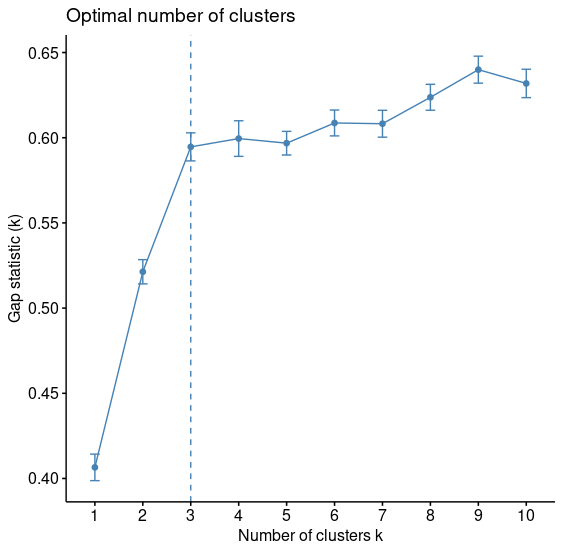
\includegraphics[width=0.46\textwidth]{~/Documents/rcw/images/Rplot09.png}
  \caption{Sillhoutte method plot}
\end{figure}

As stated previously, the \textbf{sillhoutte plot} for the data that had \textbf{PCA} done to it gives a more reasonable result for the reccomended number of clusters, this being 
\textbf{3}.

\subsection{K-means Clustering Investigation with PCA}
\subsubsection{Discussing the K-means outputs}

The most reccomended number of clusters is still \textbf{3}, however this time as the data has been passed through \textbf{PCA},
the clustering  is significantly different compared to the attempt done with the original data.
As shown in the plot below, this time there is a lot more of overlapping especially with cluster 1 and 2. This is not ideal as we want each cluster to have a clear distance 
from the other ones.
\begin{figure}[H]
  \centering
  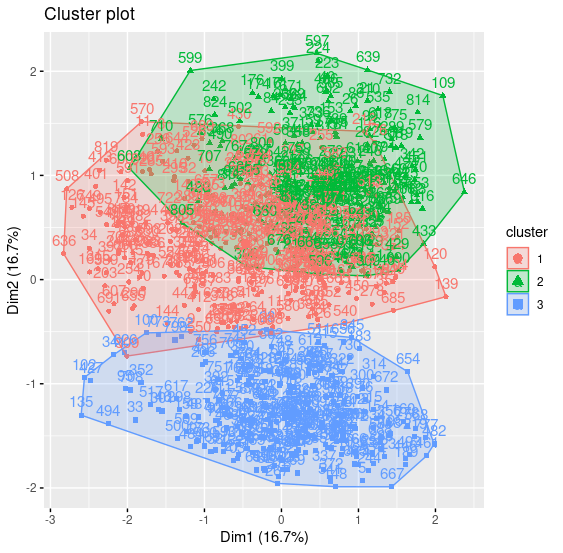
\includegraphics[width=0.8\textwidth]{~/Documents/rcw/images/Rplot10.png}
  \caption{Clustering plot}
\end{figure}
I have put below the kmeans output for the clustering attempt using the data passed through \textbf{PCA}.
I am still using \textbf{k=3} as Nbclust, elbow method and the sillhoutte plot all had an output of 3 as the best number of clusters.  
The \textbf{BSS} in this clustering is \textbf{8183.617} while the \textbf{WSS} is \textbf{5840.179}. 
The ratio of the \textbf{BSS} and the \textbf{TSS} is \textbf{58.4\%}.
By running \textbf{PCA} on the data, we were able to improve our results especially for the \textbf{WSS} as this time it is a lot lower than the original attempt.
\begin{lstlisting}
K-means clustering with 3 clusters of sizes 332, 236, 256

> kmeans_pca_data$centers
        PC1        PC2         PC3        PC4          PC5         PC6
1 -1.078026 -1.5110695  0.04723636 -0.1754898  0.009380699 -0.01659038
2 -2.911460  1.7332691  0.02469198  0.1345272 -0.123755941  0.11129772
3  4.082068  0.3618108 -0.08402257  0.1035711  0.101921914 -0.08108694

> kmeans_pca_data$cluster
  [1] 1 1 3 1 3 1 1 1 1 1 1 1 1 1 3 2 1 3 3 2 2 1 1 3 1 2 3 3 2 1 1 1 3 1 1 2 3 2 3 2 
2
 [42] 1 2 2 2 2 1 2 1 3 1 3 1 1 2 3 2 3 2 2 2 1 2 2 3 1 3 3 3 1 2 1 3 1 2 3 2 2 3 1 2 
1
 [83] 1 2 1 2 3 1 3 1 2 3 2 2 3 2 1 1 2 3 3 3 2 2 1 1 1 2 2 2 1 3 3 2 1 2 2 1 1 1 2 1 
1
[124] 3 3 1 2 3 2 1 2 1 1 2 3 2 1 3 1 1 1 1 3 1 1 3 1 3 1 2 1 1 2 3 1 1 3 3 1 3 2 2 3 
3
[165] 1 3 1 1 1 1 1 2 3 2 1 2 3 1 1 1 3 1 3 1 1 3 1 2 3 2 2 2 1 1 3 3 1 1 1 2 2 3 1 1 
1
[206] 3 2 1 2 3 2 1 3 2 3 2 2 1 3 1 3 2 2 2 2 3 1 2 1 2 3 2 1 1 2 3 2 2 1 1 3 2 2 3 2 
1
[247] 1 3 1 1 3 3 2 1 1 1 3 2 2 1 1 2 2 1 1 1 3 1 2 2 3 1 1 2 2 3 2 1 1 2 3 2 1 1 1 3 
1
[288] 3 2 1 1 3 1 1 1 2 1 3 3 3 3 3 2 1 3 2 2 2 1 2 3 3 2 3 1 2 3 2 1 1 1 3 3 2 3 3 2 
3
[329] 1 1 1 2 2 3 3 3 3 1 1 1 3 2 1 2 3 1 1 3 1 3 3 3 1 1 2 3 1 2 2 1 1 1 1 1 2 3 3 2 
2
[370] 3 2 3 2 3 1 1 1 1 3 2 1 1 1 1 1 1 1 3 1 3 1 3 1 2 2 1 1 1 2 2 1 2 3 1 1 2 1 2 3 
1
[411] 2 1 1 3 1 3 1 3 3 2 2 3 1 2 2 1 3 3 2 1 3 3 2 3 3 3 1 1 1 1 1 3 2 2 1 3 1 1 3 1 
2
[452] 3 2 2 3 3 1 1 3 3 3 2 3 3 1 1 2 3 3 1 1 2 2 3 1 2 3 3 1 2 3 3 1 3 2 2 3 3 3 2 2 
3
[493] 3 3 1 1 3 2 1 3 2 2 3 2 1 1 2 1 3 1 3 3 1 2 1 3 3 2 2 1 3 1 3 3 1 1 1 1 1 2 2 1 
1
[534] 3 2 2 1 2 3 1 3 2 2 3 3 1 3 1 1 1 3 1 2 1 3 1 1 2 3 3 3 3 1 2 2 2 3 3 3 1 3 2 1 
3
[575] 2 2 2 1 2 1 1 1 1 1 1 1 3 1 1 3 1 1 1 2 3 2 2 1 2 1 1 2 2 3 3 2 1 2 3 1 1 3 1 2 
3
[616] 2 3 2 2 1 2 1 3 3 1 3 1 1 2 1 2 3 1 3 2 1 1 1 2 1 2 1 3 1 3 2 1 1 1 1 3 1 2 3 1 
3
[657] 1 1 3 2 3 2 1 1 1 2 3 1 2 1 2 3 1 1 3 2 1 2 1 1 2 1 3 3 1 1 3 3 1 2 1 3 3 3 3 1 
3
[698] 1 1 3 3 1 3 1 3 1 2 3 1 2 3 3 3 1 2 2 3 3 3 1 3 1 1 3 1 2 1 2 1 3 1 2 1 1 1 2 3 
2
[739] 2 2 3 2 3 3 2 1 1 3 1 2 3 3 2 1 1 3 3 3 2 3 1 3 3 2 2 3 2 3 1 2 1 3 3 1 2 1 3 3 
1
[780] 1 2 1 1 3 2 1 3 2 2 3 2 1 2 2 2 1 3 3 1 2 3 1 3 3 2 1 3 2 2 1 1 3 2 2 2 1 1 1 1 
1
[821] 1 3 1 2

> kmeans_pca_data$tot.withinss
[1] 5840.179

> kmeans_pca_data$betweenss
[1] 8183.617

Within cluster sum of squares by cluster:
[1] 2415.343 1461.091 1963.745
 (between_SS / total_SS =  58.4 %)
\end{lstlisting}

\newpage
\subsubsection{Sillhoutte Plot}

From the plot below you can see that the \textbf{average width score} this time is \textbf{0.32}, this is an increase of \textbf{0.03}
as in the original attempt the score was \textbf{0.29}. Again, this is not the best result as the maximum is score \textbf{1}, but 
\begin{figure}[H]
  \centering
  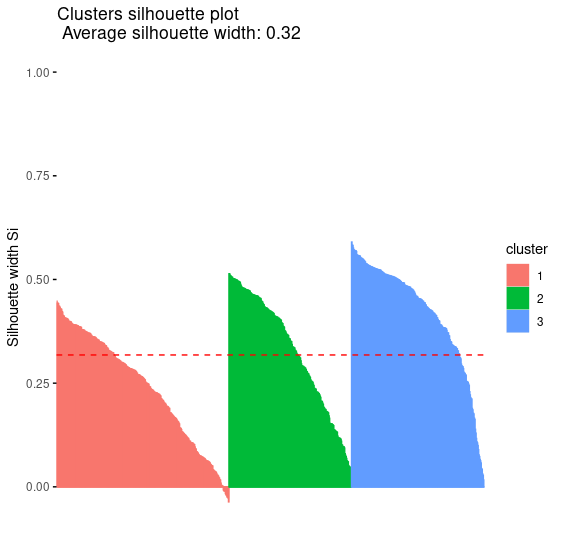
\includegraphics[width=0.5\textwidth]{~/Documents/rcw/images/Rplot11.png}
  \caption{Sillhoutte plot}
\end{figure}


\section{Energy Forecasting}


\appendix

\section{code}

\end{document}


